\documentclass[table, 12pt]{article}
\usepackage[T1]{fontenc}
\usepackage[utf8]{inputenc}
\usepackage[english]{babel}
\usepackage{graphicx}
\usepackage{titlesec}
\usepackage{hyperref}
\usepackage[usenames,dvipsnames]{xcolor}
\usepackage{float}
\usepackage[export]{adjustbox}
\usepackage{longtable}
\usepackage{mathtools}
\usepackage[most]{tcolorbox}
\usepackage{xparse}
\usepackage{subcaption}
\usepackage{listings}
\usepackage{tikz}


\hyphenation{Te-lan-ga-na}
\hyphenation{an-a-lys-ing}
\hyphenation{a-gron-o-mists}
\hyphenation{a-gron-o-mist}
\hyphenation{da-ta-base}
\hyphenation{ca-u-sed}
\hyphenation{Sen-sor-Da-ta-Ma-na-ger}
\hyphenation{Ac-count-Ma-na-ger}
\hyphenation{Lo-ca-tion-Mo-dule}
\titleformat{\paragraph}
{\normalfont\normalsize\bfseries}{\theparagraph}{1em}{}
\titlespacing*{\paragraph}
{0pt}{3.25ex plus 1ex minus .2ex}{1.5ex plus .2ex}

\def\checkmark{\tikz\fill[scale=0.4](0,.35) -- (.25,0) -- (1,.7) -- (.25,.15) -- cycle;}


% JSON style for listings
\colorlet{punct}{red!60!black}
\definecolor{background}{HTML}{EEEEEE}
\definecolor{delim}{RGB}{20,105,176}
\colorlet{numb}{magenta!60!black}

\lstdefinelanguage{shell}{
    basicstyle=\small\ttfamily,
    showstringspaces=false,
    breaklines=true,
    frame=lines,
    backgroundcolor=\color{background},
    literate=
     *{0}{{{\color{numb}0}}}{1}
      {1}{{{\color{numb}1}}}{1}
      {2}{{{\color{numb}2}}}{1}
      {3}{{{\color{numb}3}}}{1}
      {4}{{{\color{numb}4}}}{1}
      {5}{{{\color{numb}5}}}{1}
      {6}{{{\color{numb}6}}}{1}
      {7}{{{\color{numb}7}}}{1}
      {8}{{{\color{numb}8}}}{1}
      {9}{{{\color{numb}9}}}{1}
      {:}{{{\color{punct}{:}}}}{1}
      {,}{{{\color{punct}{,}}}}{1}
      {\{}{{{\color{delim}{\{}}}}{1}
      {\}}{{{\color{delim}{\}}}}}{1}
      {[}{{{\color{delim}{[}}}}{1}
      {]}{{{\color{delim}{]}}}}{1}
      {>}{{{\color{delim}{>}}}}{1},
}


\def\exampletext{Example}

\NewDocumentEnvironment{testexample}{ O{} }
{
\colorlet{colexam}{teal!60!black} % Global example color
\newtcolorbox[use counter=testexample]{testexamplebox}{%
    % Example Frame Start
    empty,% Empty previously set parameters
    title={\exampletext #1},% use \thetcbcounter to access the testexample counter text
    % Attaching a box requires an overlay
    attach boxed title to top left,
       % Ensures proper line breaking in longer titles
       minipage boxed title,
    % (boxed title style requires an overlay)
    boxed title style={empty,size=minimal,toprule=0pt,top=4pt,left=3mm,overlay={}},
    coltitle=colexam,fonttitle=\bfseries,
    before=\par\medskip\noindent,parbox=false,boxsep=0pt,left=3mm,right=0mm,top=2pt,breakable,pad at break=0mm,
       before upper=\csname @totalleftmargin\endcsname0pt, % Use instead of parbox=true. This ensures parskip is inherited by box.
    % Handles box when it exists on one page only
    overlay unbroken={\draw[colexam,line width=.5pt] ([xshift=-0pt]title.north west) -- ([xshift=-0pt]frame.south west); },
    % Handles multipage box: first page
    overlay first={\draw[colexam,line width=.5pt] ([xshift=-0pt]title.north west) -- ([xshift=-0pt]frame.south west); },
    % Handles multipage box: middle page
    overlay middle={\draw[colexam,line width=.5pt] ([xshift=-0pt]frame.north west) -- ([xshift=-0pt]frame.south west); },
    % Handles multipage box: last page
    overlay last={\draw[colexam,line width=.5pt] ([xshift=-0pt]frame.north west) -- ([xshift=-0pt]frame.south west); },%
    }
\begin{testexamplebox}}
{\end{testexamplebox}\endlist}


\begin{document}
\begin{titlepage}
    \centering
    {\scshape\large AY 2021/2022 \par}
    \vfill
    
\includegraphics[width=100pt]{assets/logo-polimi-new.pdf}\par\vspace{1cm}
    {\scshape\LARGE Politecnico di Milano \par}
    \vspace{1.5cm}
    {\huge\bfseries Implementation Document \par}
    \vspace{2cm}
    {\Large {Ottavia Belotti\quad Alessio Braccini\quad Riccardo Izzo}\par}
    \vfill
    {\large Professor\par
        Elisabetta \textsc{Di Nitto}}
    \vfill
    {\large \textbf{Version 1.0}\\ \today \par}
\end{titlepage}

\hypersetup{%
    pdfborder = {0 0 0}
}

\thispagestyle{plain}
\pagenumbering{gobble}
\mbox{}
\newpage
\pagenumbering{roman}
\tableofcontents
\newpage
\pagenumbering{arabic}

\section{Introduction}
The code can be found in the official project repository on GitHub at the link: \url{https://github.com/AlessioBraccini/SE2-Belotti-Braccini-Izzo}.
\subsection{Purpose}

This document aims to describe how the implementation and integration testing have taken place.
Implementation is the last step of the DREAM application development cycle.
It also verifies that the DREAM system satisfies its functional requirements described in the RASD document.
For this reason, the testing phase has the goal to check that the critical parts of the application work in a correct way, as described in the DD document.

\subsection{Definitions, Acronyms, Abbreviations}
\begin{itemize}
    \item ACID: Atomicity-Consistency-Isolation-Durability
    \item API: Application Programming Interface
    \item CSRF: Cross Site Request Forgery
    \item DBMS: DataBase Management System
    \item DD: Design Document
    \item HTTP: HyperText Transfer Protocol
    \item JS: JavaScript
    \item ORM: Object-Relational Mapping
    \item REST: REpresentational State Transfer
    \item RASD: Requirements Analysis and Specification Document
    \item UI: User Interface
    \item URL: Uniform Resource Locator
    \item WSGI: Web Server Gateway Interface
    \item ASGI: Asynchronous Server Gateway Interface
\end{itemize}
\subsection{Revision History}
\begin{itemize}
    \item Version 1.0:
\end{itemize}
\subsection{References}
\begin{itemize}
    \item Django Framework: \url{https://www.djangoproject.com/}
    \item REST Framework: \url{https://www.django-rest-framework.org/}
    \item Vue.js: \url{https://vuejs.org/}
    \item Axios: \url{https://axios-http.com/docs/intro}
    \item Heroku: \url{https://devcenter.heroku.com/categories/reference}
    \item PostgreSQL: \url{https://www.postgresql.org/docs/14/index.html}
\end{itemize}

\newpage
\section{Development}
\subsection{Implemented Functionalities}
Given the three types of user, we decided to implement the functionalities for Policy Maker and Agronomist users. In particular:
\subsubsection*{Policy Maker}
\begin{itemize}
    \item Farmers ranking in ascending/descending order (filtered by district or global)
    \item Visualization of humidity and water irrigation sensors data through graphs
    \item Download agronomists' reports about steering initiatives
\end{itemize}
\subsubsection*{Agronomist}
\begin{itemize}
    \item Farmers ranking in ascending/descending order tailored to the agronomist's district
    \item Uploading of reports concerning steering initiatives
    \item Creation and updating of daily plans
    \item Help requests inbox
    \item Weather widget
\end{itemize}
For details about these functionalities please refer to the RASD document.

\paragraph{Not implemented functionalities}
Farmer user's functionalities have not been implemented at this stage. To take care of the farmers' lack of data, some entries has been inserted in the database to mimic the normal behaviour and let agronomist and policy maker users experience the prototype application. In particular, farmer users, help requests and sensors data have been made up.
\newpage
\subsection{Implemented Requirements}
In the following list of requirements (taken from RASD), the implemented ones are checked with a tick, while the other ones refer to the farmer user type so they have not been implemented.
\newcounter{RequirementCtr}
\begin{itemize}
    \stepcounter{RequirementCtr}
    \item[\textbf{R\arabic{RequirementCtr}.}] The system must allow only registered and logged-in users to use the app. \checkmark
    \stepcounter{RequirementCtr}
    \item[\textbf{R\arabic{RequirementCtr}.}] The system shall allow users to be identified by an email of their choosing. \checkmark
    \stepcounter{RequirementCtr}
    \item[\textbf{R\arabic{RequirementCtr}.}] The system must suggest to the farmer users the area in which they are during the registration phase if the IT device is equipped with GPS technology. In any case, the final decision will be up to the registering user. $\times$
    \stepcounter{RequirementCtr}
    \item[\textbf{R\arabic{RequirementCtr}.}] The system must inform the user to try later if they are experimenting connectivity issues. \checkmark
    \stepcounter{RequirementCtr}
    \item[\textbf{R\arabic{RequirementCtr}.}] The system must allow Policy Makers to see up-to-date statistic data, accordingly to the database, about water irrigation systems and soil humidity sensors. \checkmark
    \stepcounter{RequirementCtr}
    \item[\textbf{R\arabic{RequirementCtr}.}] The system must allow Policy Makers to retrieve all agronomists' steering initiative reports uploaded to the database. \checkmark
    \stepcounter{RequirementCtr}
    \item[\textbf{R\arabic{RequirementCtr}.}] The system must give Policy Makers up-to-date ranking of the best and worst performing farmers. \checkmark
    \stepcounter{RequirementCtr}
    \item[\textbf{R\arabic{RequirementCtr}.}] The system must use a fair and scientific score to rank the Farmers in order to represent the real situation. $\times$
    \stepcounter{RequirementCtr}
    \item[\textbf{R\arabic{RequirementCtr}.}] The system must let Farmers insert their production information every day. $\times$
    \stepcounter{RequirementCtr}
    \item[\textbf{R\arabic{RequirementCtr}.}] The system must provide the contact of the agronomist appointed to the area of the Farmer requesting professional help. $\times$
    \stepcounter{RequirementCtr}
    \item[\textbf{R\arabic{RequirementCtr}.}] The system must allow every user registered as Farmer to access the forum, to create new discussions and to post replies to already existing ones.
    \stepcounter{RequirementCtr} $\times$
    \item[\textbf{R\arabic{RequirementCtr}.}] The system must notify Agronomists of unresolved requests of help from Farmers. \checkmark
    \stepcounter{RequirementCtr}
    \item[\textbf{R\arabic{RequirementCtr}.}] The system must allow the Agronomists to add a new schedule for the day each day. \checkmark
    \stepcounter{RequirementCtr}
    \item[\textbf{R\arabic{RequirementCtr}.}] The system must suggest to the Agronomists which farms to visit while planning the Daily Plan based on the number of received visits. \checkmark
    \stepcounter{RequirementCtr}
    \item[\textbf{R\arabic{RequirementCtr}.}] The system must suggest to the Agronomists only the farms among the ones in their competence area. \checkmark
    \stepcounter{RequirementCtr}
    \item[\textbf{R\arabic{RequirementCtr}.}] The system must allow the Agronomists to update their schedule during the day. \checkmark
    \stepcounter{RequirementCtr}
    \item[\textbf{R\arabic{RequirementCtr}.}] The system must register the already uploaded schedule as definitive at 23:59 of the current day. \checkmark
    \stepcounter{RequirementCtr}
    \item[\textbf{R\arabic{RequirementCtr}.}] The system must give Agronomists up-to-date ranking of the best and worst performing farmers in their responsibility area. \checkmark
    \stepcounter{RequirementCtr}
    \item[\textbf{R\arabic{RequirementCtr}.}] The system must show weather forecasts relevant to the area concerning the Farmer or the Agronomist. \checkmark
    \stepcounter{RequirementCtr}
    \item[\textbf{R\arabic{RequirementCtr}.}] The system must present news concerning crop only if relevant to the Farmer's own crop type. $\times$
    \stepcounter{RequirementCtr}
    \item[\textbf{R\arabic{RequirementCtr}.}] The system must allow Policy Makers to upload their steering initiative reports to the database. \checkmark
\end{itemize}

\subsection{Design Choices}
We would like to point out that the prototype's UI has been designed mainly for mobile browsing, because it is more comfortable to use a smartphone on the field from a farmer's perspective. However, it is completely functional on laptops and computers too, even if it's a little less pleasing to the eye.

\subsection{Adopted Development Frameworks}
The chosen frameworks, for both frontend and backend developing, inherently force the standard and well suited architectural patterns. In particular, Django Framework forces a \emph{Model-View-Controller} (MVC) while Vue.js a \emph{Model-View-ViewModel} (MVVM) which is a declination of the MVC pattern, which is better suited for frontend development. 

\paragraph{MVC} In the MVC pattern, the \textbf{model} is the one in charge of defining the data storage, the \textbf{view} is majorly associated with the User Interface (UI) and it is used to provide the visual representation of the MVC model, also handling the communication between the user (inputs, requests, etc.) and the controller, while the \textbf{controller} is the connection between models and views.

\paragraph{MVVM} In the MVVM pattern, the \textbf{model} is the data access layer and represents real state content. The \textbf{views} displays a representation of the model and receives the user's interaction with the view. Both of these are as in the MVC pattern. While, the \textbf{view-model} is an abstraction of the view exposing public properties and commands. Instead of the controller of the MVC pattern, the MVVM has a \textbf{binder} which automates communication between the view and its bound properties in the view model.
\paragraph{}
All in all, the advantages of using MVC (and similarly MVVM) can be summed up as: 
\begin{itemize}
    \item The \textbf{structured organization} that helps managing large applications, making the design choice more scalable
    \item The support for the invocation of \textbf{asynchronous methods}, making the backend and frontend integration very fast and dynamic
    \item \textbf{Easy to modify}, making it suited to further develop the project, even after this prototype, without affecting the already present architecture, easing the mantainment
    \item Allows \textbf{test-driven development}, since it simplifies the testing process
\end{itemize}

\begin{figure}[H]
    \subfloat{{
\includegraphics[scale=0.05]{assets/Django-Logo.png}}}%
    \qquad
    \subfloat{{
\includegraphics[scale=0.4]{assets/Rest-Logo.png}}}%
    \caption{Django Framework and REST Framework logo}
\end{figure}
\begin{center}
    \begin{figure}[H]
        
\includegraphics[scale=0.65, center]{assets/Vue-Logo.png}
        \caption{Vue.js Framework logo}
        \label{fig: vue_logo}
    \end{figure}
\end{center}

\subsubsection{Programming Language}
The programming language of choice for DREAM's backend is \textbf{Python}, an interpreted high-level general-purpose programming language, supporting multiple programming paradigms.

For what concerns DREAM's development requirements, Python has more advantages than disadvantages.
\begin{itemize}
    \item \textbf{Pros:}
    \begin{itemize}
        \item[+] \textbf{Allow fast development}: Python is a very high-level programming language, so the built-in functions and reliable third-parties libraries allow us to spend the development time focusing on implementing the desired custom behaviors rather than building basic and non-functional features that are shared among most web apps.
        \item[+] \textbf{Readability}: Python's syntax is very clear and human-friendly.
        \item[+] \textbf{Large community and widely spread among WebApps}: being used a lot by the web app developers' community, the internet is full of help for troubleshooting. Moreover, this has resulted in very extensive support through libraries dedicated to web development and integration with frontend frameworks.
    \end{itemize}
    \item \textbf{Cons:}
    \begin{itemize}
        \item[-] \textbf{Speed}: being an interpreted language, Python suffers of slower computation in comparison to other compiled languages (e.g. C++, Java, etc.).
    \end{itemize}
\end{itemize}

For the client side we chose \textbf{JavaScript}, a text-based programming language, that allows to build interactive web pages. It handles the user's interaction with the elements present on the page.
Alongside JavaScript, we used HTML and CSS to give structure and style to the page.

\subsubsection{Django Framework}
Django is a Python web framework which aims for rapid development without sacrificing well structured code. In fact, the framework encourages to follow the MVC pattern and embeds it into its Django apps structure.

It is \textbf{secure}, since it provides the developers security tools (e.g. automatic users' password encryption, CSRF protection, SSL/HTTPS support, etc.) that have been implemented by experts in the field. See more about security in section \ref{REST}.

It is \textbf{supportive}, given that it has lots of database operation support thanks to the \emph{Object-relational mapping} (ORM) feature which easily maps DB tables to \emph{Django Model} components (Model in MVC pattern) within the code, basic queries can be done transparently and in a very readable fashion without losing in performance.
Moreover, it allows to configure the \emph{Admin Interface} from where authorized users can easily manage the database, like monitoring at a glance the entries in all the DB tables and create new ones for testing purposes. Apart from the DB integration,  Django allows the creation of custom \emph{endpoint URLs} from where the frontend will make the backend calls. Meanwhile the \emph{Django View} components come to be a dedicated place for managing HTTP requests, acting as the Controller in MVC design. Django can also support \emph{Template} components as its Views in MVC pattern, but in this project they haven't been used because of the different framework choice to handle the representation part (see section \ref{Vue}).

Furthermore, Django is \textbf{extensively documented} and \textbf{scalable} since it's being used in very demanding professional contexts, being one of the frameworks of choice of well known social media platforms that experience high loads of requests due to their intensive usage from their user base.

\paragraph{Django Middlewares}
To manage the communication between backend and frontend, we mainly use the following Django middlewares:
\begin{itemize}
    \item \textit{SecurityMiddleware}
    \item \textit{SessionMiddleware}
    \item \textit{CsrfViewMiddleware}
    \item \textit{AuthenticationMiddleware}
\end{itemize}

Furthermore, since we used Django REST Framework, the \textit{CorsMiddleware} is the one dealing with the message exchanges between frontend and backend (i.e. POST and GET).

\subsubsection{Django REST Framework}
\label{REST}
We decided to pair REST framework to our Django backend since REST allows even more security features.

We used its authentication policies, in particular the \textbf{REST Token-based authentication} that ensures an authorized clients' connection to the backend, so that every interaction with the application server is safe from an authentication point of view: unknown users can access none of the backend's functionalities.

We used the \emph{Djoser} REST library to handle user login and signup. The choice has been made to make sure that such standard operations are carried out without flaws, especially in handling sensitive data (i.e. passwords). Moreover, \emph{Djoser} is compatible with custom User Models, so it enables us to delegate the authentication phase to it even with our custom User model.

Furthermore, Django REST gives an extensive support in building \emph{Django Views}, from basic skeleton function (\texttt{@api\_view}) for managing all types of HTTP requests, up to more functional and request-specific functionalities.

\subsubsection{Vue.js}
\label{Vue}
Vue.js is a famous frontend JavaScript framework that allow the creation of user interfaces and single-page applications.
The core library is focused on the view layer only.
Advanced features required for complex applications such as routing, state management and build tooling are offered via officially maintained supporting libraries and packages.

We used this framework to build up the client-side rendering of pages because of the easy usability as it integrates, in a single .vue file (also called components),
the three main blocks of a web application paradigm.

The structure of a Vue file is intuitive, it is composed by three blocks:
\begin{itemize}
    \item HTML: the part where the structure of the component is created.
    \item JavaScript: the part where interactive elements are placed, or better the logic, of the component.
    \item CSS: the part where the style of the HTML structure is placed, it can be scoped to the actual component or not.
\end{itemize}
In order to communicate with the backend we use the JavaScript library Axios that is a promise-based HTTP Client for Node.js.
On the server-side it uses the native Node.js http module, while on the client it uses XMLHttpRequests.
Axios' killer feature is that it can transform in an automatic way the json reply that arrives from the server in JavaScript ready XMLHttpRequests.

\subsection{API Integration}
\subsubsection{OpenWeatherMap API}
To allow the user to retrieve the weather information we use this external api service that lets us know in real time
the weather condition of a specific place in the world.
This returns us not only the basics information, but also more specific ones like pressure or wind speed and direction.

\subsection{DataBase}
Our database system of choice is PostgreSQL, a well known object-relational database. It is reliable, robust, ACID-compliant and ensures high performance. 
Furthermore it is supported excellently by Django.

\subsection{Heroku}
We choose to host our project in a server in order to make it reachable by everyone
that has a browser and an internet connection.
The hosting service that we have chosen is Heroku, a platform as a service (PaaS)
that enables developers to build, run, and operate applications entirely
in the cloud.

We created two different servers, one for the backend and one for the frontend.
Heroku also gives the possibility to register a custom subdomain to reach the
website
We choose:
\begin{itemize}
    \item \url{dreamapplication.herokuapp.com} as frontend domain
    \item \url{appdream.herokuapp.com} as backend domain
\end{itemize}



\section{Source Code}
\subsection{Backend Structure}
\begin{center}
    \begin{figure}[H]
        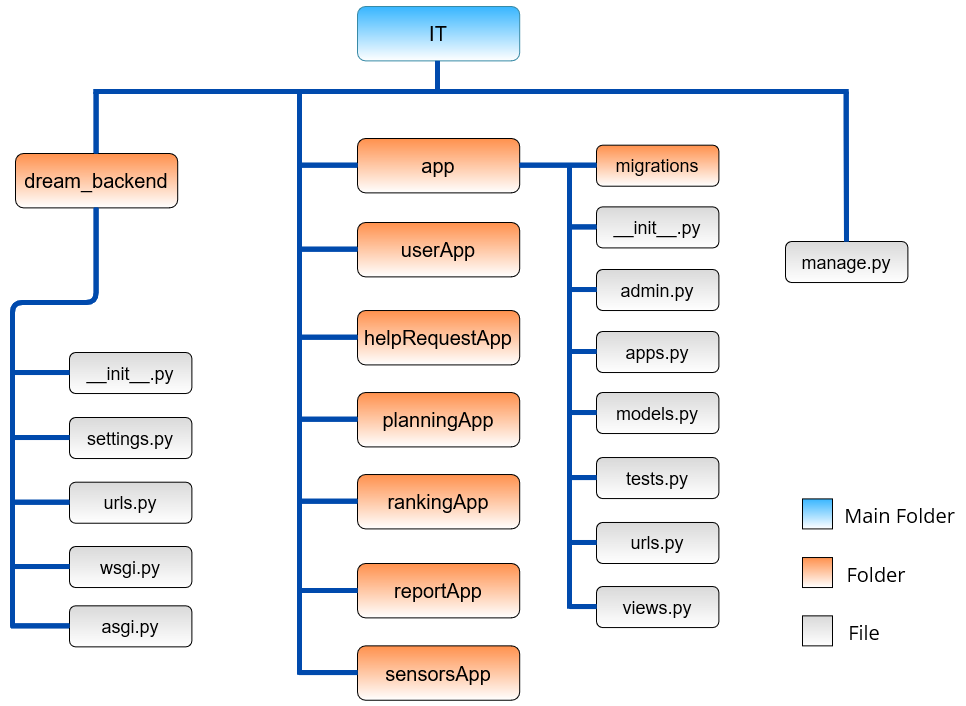
\includegraphics[scale=0.65, center]{assets/backend_structure.png}
        \caption{Backend structure}
        \label{fig: backend_structure}
    \end{figure}
\end{center}

The backend of the application follows the common Django project structure as shown in the figure above.
This section describes the structure of the project and the role of each app.\newline
Here is the structure of the backend:

\begin{itemize}
    \item \textbf{IT}: root directory, container for the project
    \item \textbf{dream\_backend}: folder that contains the configuration files of the project
    \item \textbf{\_\_init.py\_\_}: it tells the Python interpreter that the directory is a Python package
    \item \textbf{settings.py}: main setting file for the Django project, used to configure all the applications and middleware, it also handles the database settings
    \item \textbf{urls.py}: URL declarations for the Django project, it contains all the endpoints that the website should have
    \item \textbf{wsgi.py}: entry-point for WSGI-compatible web servers to serve your project, it describes the way in which servers interact with the applications
    \item \textbf{asgi.py}: entry-point for ASGI-compatible web servers to serve your project, ASGI works similar to WSGI but comes with some additional functionality
    \item \textbf{migrations}: Django's way of propagating changes to the models into the database schema, when changes occur this folder is populated with the records of them
    \item \textbf{admin.py}: used for registering the Django models into the Django administration, it allows to display them in the Django admin panel
    \item \textbf{apps.py}: common configuration file for all Django apps, used to configure the attributes of the app
    \item \textbf{models.py}: it defines the structure of the database, it allows the user to create database tables for the app with proper relationships using Python classes. It tells about the actual design, relationships between the data sets and their attribute constraints
    \item \textbf{tests.py}: used to test the overall functionality of the app through unit tests
    \item \textbf{views.py}: provide an interface through which a user interacts with a Django website, it contains the business logic of the app
    \item \textbf{manage.py}: command-line utility for executing Django commands; these includes debugging, deploying and running
\end{itemize}

\begin{center}
    \begin{figure}[H]
        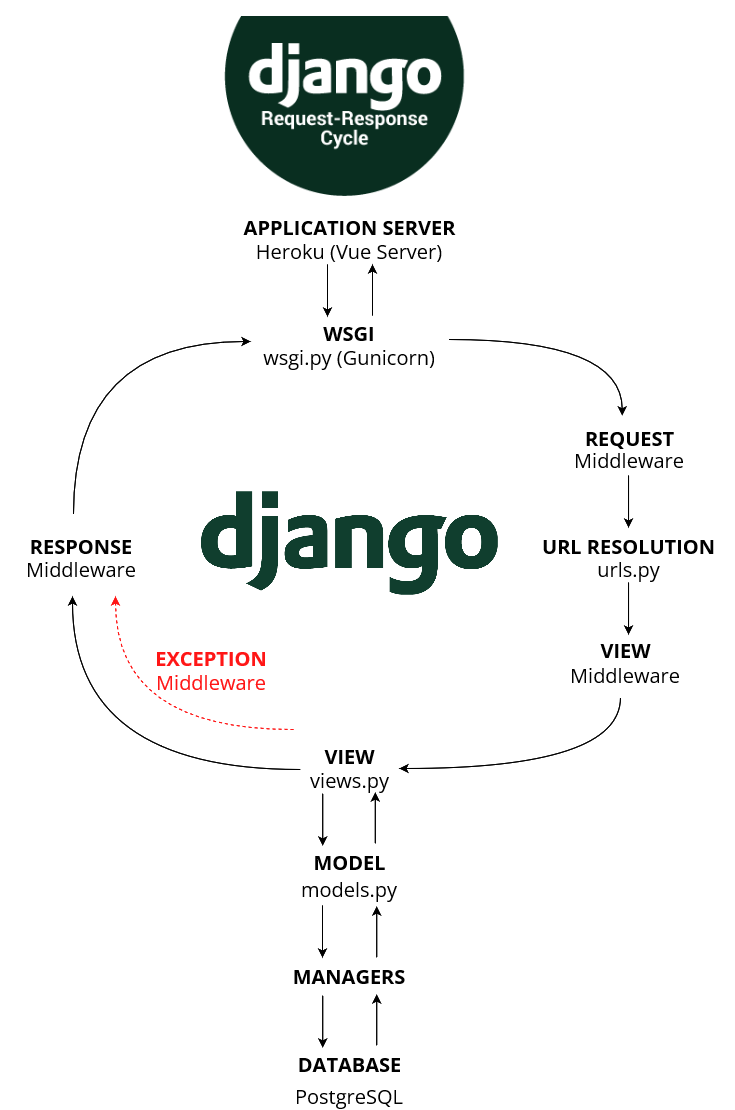
\includegraphics[scale=0.55, center]{assets/django_request_response_flow.png}
        \caption{Django Request-Response Cycle}
        \label{fig: django_flow}
    \end{figure}
\end{center}

All the functionalities of the website are managed by different apps, these are the ones implemented:
\begin{itemize}
    \item \textbf{app}: implements common functionalities that cover the entire application, it has one endpoint:
    \begin{itemize}
        \item[--] \textbf{farms\_list}: handled by \textit{FarmView} view, it manages GET requests by returning a list of farms
    \end{itemize}
    \item \textbf{userApp}: implements the custom authentication system of the application, it contains all the models regarding the user. It has one endpoint that is used to check if a user is authenticated or not
    \item \textbf{helpRequestApp}: implements the functionalities about the help requests with two endpoints:
    \begin{itemize}
        \item[--] \textbf{help\_request}: handled by \textit{HelpRequests} view, it manages GET requests by returning the list of help requests and POST requests to reply to an existing requests
        \item[--] \textbf{help\_request\_by\_id}: handled by \textit{HelpRequestByID} view, it manages GET requests by returning a single help request associated to the unique id specified as a parameter
    \end{itemize}
    \item \textbf{planningApp}: implements the functionalities about the daily plan with two endpoints:
    \begin{itemize}
        \item[--] \textbf{daily\_plan}: handled by \textit{DailyPlanView} view, it manages GET requests by returning the list of dates for the daily plan and POST requests to upload a new daily plan
        \item[--] \textbf{update\_daily\_plan}: handled by \textit{UpdateVisits} view, it manages GET requests by returning the list of farmers in the current daily plan and POST requests to perform an update of an already existing daily plan
    \end{itemize}
    \item \textbf{rankingApp}: implements the functionalities about the ranking with two endpoints:
    \begin{itemize}
        \item[--] \textbf{rank\_farmers}: handled by \textit{RankFarmers} view, it manages GET requests by returning the ranking as a list of farmers
        \item[--] \textbf{profile\_info}: handled by \textit{ProfileFarmers} view, it manages GET requests by returning the profile info of a selected farmer
    \end{itemize}
    \item \textbf{reportApp}: implements the functionalities about the steering initiatives with two endpoints:
    \begin{itemize}
        \item[--] \textbf{steering\_initiatives}: handled by \textit{SteeringInitiativeView} view, it manages GET requests by returning the list of reports uploaded to the app and POST requests to upload a new report
        \item[--] \textbf{download\_reports}: handled by \textit{DownloadReport} view, it manages GET requests by returning a specific reports based on some parameters
    \end{itemize}
    \item \textbf{sensorsApp}: implements the functionalities about the sensors (humidity and water irrigation) with two endpoints:
    \begin{itemize}
        \item[--] \textbf{humidity}: handled by \textit{Humidity} view, it manages GET requests by returning a list with humidity and temperature values for each district
        \item[--] \textbf{water\_irrigation}: handled by \textit{WaterIrrigation} view, it manages GET requests by returning a list of water quantity values for each district
    \end{itemize}
\end{itemize}

\subsection{Frontend Structure}

The frontend web app is contained into the \textit{dream\_frontend/dream\_app} folder of
the IT directory.
Of course, following the four tier architecture described in the Design Document,
the frontend web application can also be deployed to a dedicated web server,
which will then make requests to a different backend server.
Here is represented the structure of the web app:
\begin{itemize}
    \item \textbf{node\_modules}: here all the installed dependencies of the project, listed in the \textit{package.json} file, are stored.
    It's generated automatically every time the project is set up.
    \item \textbf{public}: in this folder the \textit{index.html} file is present, where all the generated code will be injected in order to display it on the browser.
    During the building phase the files in this directory don't change.
    \item \textbf{src}: this is the main folder of the project. It is divided in several subfolders:
    \begin {itemize} 
        \item \textbf{assets}: it contains all the images needed by the frontend like the icons of the weather or the logo in the login page.
        \item \textbf{router}: it contains the JavaScript file that list all the routes used to navigate the frontend.
        \item \textbf{views}: it contains all the vue components needed by the frontend.
        They are divided in category, e.g. Policymaker or Agronomist, in order to better separate the different logic.
    \end{itemize}
\end{itemize}

There are other several files needed by Vue to run the project. The most important are:
\begin{itemize}
    \item \textbf{package.json}: it contains the list of all the dependencies installed in the project.
    \item \textbf{server.js}: a simple JavaScript file needed by Heroku in order to start the web server and accept the incoming requests.
    \item \textbf{config.js}: it contains the url of the backend server.
    It can be set by the final user in order to specify if the server has to run local or online.
\end{itemize}

When the build process is finished, the web-ready files are put in the \textit{dist} directory.

\newpage
\section{Testing}

In this section we described how we tested the application following the general guidelines given in the Design Document.
The testing process has been divided into unit testing, system testing and post-deployment testing.
We decided to test only the backend because most of the logic resides here.
In any case, the system testing and the post-deployment testing phases also covered the functioning of the frontend.

\subsection{Unit Testing}
For each app in the backend we wrote the test cases in tests.py file using \textbf{unittest}, a built-in module from the Python standard library.
\subsubsection*{helpRequestApp}
\begin{itemize}
    \item Attempt to get the list of help requests by a user through a GET request on \textit{help\_request} endpoint
    \item Attempt to get the list of help requests in case of an invalid user
    \item Attempt to reply to an existing help request through a POST request on \textit{help\_request} endpoint, verify the correct deletion of the old help request which is replaced by the reply
    \item Attempt to reply to an existing help request in case of an invalid user
    \item Attempt to get a single help request given the id through a POST request on \textit{help\_request\_by\_id} endpoint
    \item Attempt to get a single help request given the id in case of an invalid user
\end{itemize}
\subsubsection*{planningApp}
\begin{itemize}
    \item Attempt to upload a new daily plan through a POST request on \textit{daily\_plan} endpoint
    \item Attempt to upload a new daily plan with an invalid region
    \item Attempt to upload a new daily plan with an invalid date
    \item Attempt to upload a new daily plan with an duplicated farmer
    \item Attempt to upload a new daily plan with an invalid user (not an agronomist)
    \item Attempt to retrieve the daily plans through a GET request on \textit{daily\_plan} endpoint
    \item Attempt to retrieve only the daily plans associated to the current user
    \item Attempt to update a daily plan through a POST request on \textit{update\_daily\_plan} endpoint
    \item Attempt to update an old daily plan
    \item Attempt to remove a daily plan
    \item Attempt to update a daily plan before creating it
\end{itemize}
\subsubsection*{rankingApp}
\begin{itemize}
    \item Attempt from an agronomist to get the ranking in "descending" order specified in the parameters through a GET request on \textit{rank\_farmers} endpoint
    \item Attempt from an agronomist to get the ranking in "ascending" order specified in the parameters
    \item Attempt from a policymaker to get the ranking in "descending" order and district among the parameters
    \item Attempt from a policymaker to get the ranking in "ascending" order and district among the parameters
    \item Attempt from a policymaker to get the ranking in different districts
    \item Attempt from a policymaker to get the ranking in "ascending" order but without the district among the parameters
    \item Attempt from a policymaker to get the ranking in "descending" order but without the district among the parameters
    \item Attempt to get informations about a farmer in the ranking through a GET request on \textit{profile\_info} endpoint
    \item Attempt to get informations about a farmer in the ranking in case of an invalid user
\end{itemize}
\subsubsection*{reportApp}
\begin{itemize}
    \item Attempt from an agronomist to upload a new report through a POST request on \textit{steering\_initiatives} endpoint
    \item Attempt from a policymaker to upload a new report
    \item Attempt to upload duplicated reports
    \item Attempt to get the list of reports through a GET request on \textit{steering\_initiatives} endpoint
    \item Attempt to get a report that has been deleted
\end{itemize}
\subsubsection*{sensorsApp}
\begin{itemize}
    \item Attempt to get data about humidity sensors through a GET request on \textit{humidity} endpoint
    \item Attempt to get data about water irrigation sensors through a GET request on \textit{water\_irrigation} endpoint
\end{itemize}

There is a total of 32 tests with a percentage of success of 100\%, this establishes the stability of the system.
All the tests can be verified by running "python manage.py test" in the root directory.

\subsection{System Testing}
A part of the testing phase was also dedicated by manually testing the app through the web browser and with Postman, a tool for generating HTTP GET/POST requests with custom parameters and inspect the backend server replies.
In this way we tested the authentication phase and all the functionalities provided by the system.
All the tests have been performed successfully.

\subsection{Post-deployment Testing}
After the deploy, the application has been extensively tested. This allowed to test the entire system and the interactions between the components both on frontend and backend.
We also invited a couple of testers in order to stress the app.


\section{Installation}
As a web application we chose to deploy it on Heroku, so
a fully running version of the software is available at:\newline
\url{https://dreamapplication.herokuapp.com/}.

We strongly suggest you to use the deployed version instead of installing the software locally, since this would require some changes both in backend and frontend source code.
Mind that, running the backend locally requires some adjustments to deal with static files. In fact, to be able to deploy the backend on a Cloud Application Platform such as Heroku, the storage of static files (i.e. Steering Initiatives reports uploaded by agronomists) has been managed through Google Drive. 

However, if you wish to install it on your machine you can follow the guide below. 

\subsection{Requirements}
\textbf{Node.js} is required in order to run the frontend, install it if you don't
have it on your device.

To run the backend, \textbf{Python 3.10} or a compatible version is mandatory. Moreover, the \texttt {\textbf{pip}} command must be installed too, in order to resolve the project's dependencies. 

A \textbf{PostgreSQL database} must be set and running as well.

\begin{itemize}
    \item \textbf{Python and Pip}
    \begin{itemize}
        \item Download Python 3.10 or equivalent from \url{https://www.python.org/downloads/}
        \item Install the latest version of Pip referencing \url{https://pip.pypa.io/en/stable/installation/}
    \end{itemize}
    \item \textbf{Node.js}
    \begin{itemize}
        \item Download the latest version of Node.js \url{https://nodejs.org/it/download/}
    \end{itemize}
    \item \textbf{PostgreSQL}
    \begin{itemize}
        \item Download the installer of the latest version from \url{https://www.postgresql.org/download/} for your OS
    \end{itemize}
\end{itemize}

\subsection{Backend Installation}
\begin{itemize}
    \item[1)] Download the latest zip archive from the Releases section on the project's GitHub repository
    \item[2)] Extract all the files in the same folder
    \item[3)] Create a \texttt{.env} file in the same folder with the following fields and fill it:
    \begin{itemize}
        \item[\textit{i.}] \texttt{SECRET\_KEY} is the key used by Django to manage authentication and hashing messages. You can set your own.
        \item[\textit{ii.}] \texttt{DATABASE\_NAME}, \texttt{DATABASE\_USER} and \texttt{DATABASE\_PWD} are credential to access your local PostgreSQL database. If you wish to use a non-local PostgreSQL database, you can also provide the \texttt{DATABASE\_URL} variable.
        \item[\textit{iii.}] \texttt{LOCAL\_STATIC\_FILES} can be set either to \texttt{True} or \texttt{False} to indicate if you want to store static files locally or on Google Drive.
        \begin{itemize}
            \item If \texttt{True} (or not set), then the \emph{Steering Initiatives} reports uploaded to the app will be stored in 'generated/reports'
            \item If \texttt{False}, then the reports are going to be stored on Google Drive (refer to next point)
        \end{itemize} 
        \item[\textit{iv.}] \texttt{GOOGLE\_DRIVE\_STORAGE\_JSON\_KEY\_FILE\_CONTENTS} and \texttt{GOOGLE\_\\DRIVE\_STORAGE\_SERVICE\_MAIL} must be set if \texttt{LOCAL\_STATIC\_\\FILES=false}. This happens because a Google Drive API is going to be used to store static files. You have to:
        \begin{itemize}
            \item Create a service account on a project in Google Developers Console: this will be your service email
            \item Generate a secret service key and store it in a safe place. Copy and paste its content in the JSON Key variable
        \end{itemize}      
    \end{itemize}
    \begin{lstlisting}[language=shell]
SECRET_KEY=your_backend_secret_key

DATABASE_NAME=your_database_name
DATABASE_USER=your_database_admin_username
DATABASE_PWD=your_database_password

LOCAL_STATIC_FILES=true/false

# if LOCAL_STATIC_FILE=false then the following variables must be set as well
GOOGLE_DRIVE_STORAGE_JSON_KEY_FILE_CONTENTS={your_JSON_key_file_content_for_Google_Drive_API}
GOOGLE_DRIVE_STORAGE_SERVICE_EMAIL=your_project.iam.gserviceaccount.com
    \end{lstlisting}  
    \item[4)] Save \texttt{.env}
    \item[5)] Make sure you have your PostgreSQL database ready and running
    \item[6a)] If you are on a Unix-like system (Linux-Debian or MacOS) with bash/zsh shell, you can run the Makefile in the \textit{dream\_pkg} via \texttt{make run} command: this will install all the dependencies, update the database schema and start the backend server. However, if you wish to do that manually, you can follow the commands below:
    \begin{lstlisting}[language=shell]
# create virtual environment
dream_pkg:~$ python3 -m venv IT/venv

# activate venv
dream_pkg:~$ source IT/venv/bin/activate

# install dependencies
dream_pkg:~$ pip install -r IT/requirements.txt

# update database schema
dream_pkg:~$ python3 IT/manage.py makemigrations
dream_pkg:~$ python3 IT/manage.py migrate

# start backend server
dream_pkg:~$ python3 IT/manage.py runserver
    \end{lstlisting}
    \item[6b)] If you are on Windows, run the following commands:
    \begin{lstlisting}[language=shell]
# create a new virtual environment
C:\dream_pkg\> python -m venv c:\dream_pkg\IT\venv

# activate venv: 2 options
C:\dream_pkg\> IT\venv\Scripts\activate.bat  #for cmd.exe
PS C:\dream_pkg\> IT\venv\Scripts\Activate.ps1  #for PowerShell
  
# install dependencies
C:\dream_pkg\> pip install -r IT\requirements.txt

# update database schema
C:\dream_pkg\> python IT/manage.py makemigrations
C:\dream_pkg\> python IT/manage.py migrate

# start backend server
C:\dream_pkg\> python IT/manage.py runserver
    \end{lstlisting}
\end{itemize}

\subsection{Frontend Installation}
Firstly, you have to specify in the config.js file (contained in \newline \textit{IT/dream\_frontend/dream\_app}) if you want to run the backend online or locally on your device.
Inside the file you will find a configuration string and you have to insert the url of the chosen backend
(by default it is set to the online backend but some choices are already available).

\begin{itemize}
    \item [1] Open a terminal and move to \textit{dream\_app} folder
    \item [2] Run \texttt{npm install} command
    \item [3] Run \texttt{serve dist} command to start the frontend server
    \item [4] Follow the instructions
\end{itemize}

The process will install the needed node modules and build the project automatically.
If you want to build it by yourself you can use this command: \texttt{npm run build}.

\section{Effort Spent}
\begin{tabular}{|c||c|}
    \hline
    Student & Time for implementation\\ \hline
    Ottavia Belotti & 80h\\
    Alessio Braccini & 80h\\
    Riccardo Izzo & 80h\\
    \hline
\end{tabular}

\end{document}

